\chapter{Studi Literatur}

Pada bab ini, akan diisi oleh studi literatur, hal-hal yang berkaitan dengan topik persoalan tugas akhir akan dipaparkan dalam bab ini guna untuk memberikan informasi mengenai dasar teori dan studi yang dipakai. Bab ini diharapkan membantu pembaca untuk mengerti dalam membaca penelitian tugas akhir ini.

\section{\textit{Information Retrieval}}
\textit{Information Retrieval} (IR) adalah proses mencari bahan, biasanya berbentuk dokumen, yang bersifat tak terstruktur, biasanya teks, yang memenuhi kebutuhan informasi dari dalam koleksi besar \parencite{introtoinforetri}. IR saat ini sangat sering dilakukan contohnya dalam pencarian informasi berkaitan dengan representasi, penyimpanan, pengaturan, dokumen, halaman web, katalog online, catatan, dan objek multimedia. 

Tujuan utama dari IR adalah penyediaan akses yang efektif dan efisien ke informasi yang dibutuhkan oleh pengguna dalam situasi tertentu. Pengguna IR dapat beragam seperti individu, organisasi, maupun sistem yang membutuhkan informasi yang relevan. IR melibatkan penggunaan teknik-teknik seperti \textit{indexing, searching, retrieval,} dan \textit{evaluation} untuk memastikan informasi yang dihasilkan relevan, tepat, dan sesuai dengan kebutuhan pengguna.

Biasanya IR tersusun oleh beberapa komponen, diantaranya.
\begin{enumerate}
    \item \textit{Indexing}, proses mengubah dokumen menjadi bentuk yang lebih mudah dicari oleh sistem IR.
    \item \textit{Searching}, proses pencarian yang dilakukan oleh pengguna dengan memberikan \textit{query} ke dalam sistem IR dan sistem memberikan keluaran berupa dokumen yang paling relevan.
    \item \textit{Retrieval}, proses sistem IR mengambil dokumen yang relevan dan mengurutkan dokumen berdasarkan kesesuaian dengan \textit{query}.
    \item \textit{Evaluation}, proses penilaian kualitas sistem IR yang biasanya mencakup metrik evaluasi seperti \textit{precision}, \textit{recall}, dan skor F1. 
\end{enumerate}

Dalam melakukan proses-proses tersebut, komponen tersebut menggunakan beberapa teknik, diantaranya.
\begin{enumerate}
    \item \textit{Term Weighting}, teknik pemberian bobot terhadap kata-kata untuk membedakan yang lebih penting dan yang kurang.
    \item \textit{Query Expansion}, teknik menambahkan kata-kata yang relevan pada \textit{query} pengguna untuk meningkatkan akurasi hasil pencarian.
    \item \textit{Clustering}, teknik mengelompokkan dokumen yang mirip untuk memudahkan pengambilan.
\end{enumerate}

\section{Apache Lucene}
Apache Lucene adalah sebuah perpustakaan atau library open-source untuk Information Retrieval (IR) atau pencarian informasi yang berbasis teks. Lucene adalah \textit{library search engine} yang berperforma tinggi dan berfitur lengkap. Lucene cocok untuk aplikasi yang memerlukan pencarian terstruktur, pencarian teks lengkap, pencarian pada graf dengan banyak node maupun vektor derajat tinggi, koreksi ejaan, atau saran kueri \parencite{apachelucene}. Lucene dikembangkan di bahasa pemrograman Java dan berfokus pada pencarian teks di dalam dokumen.

Lucene menggunakan model inverted index untuk mempercepat proses pencarian. Model ini mengubah dokumen yang diberikan menjadi indeks kata kunci atau \textit{term} dan menunjukkan letak setiap kata kunci tersebut muncul dalam dokumen. Indeks akan digunakan oleh Lucene untuk mencari kata kunci tertentu dalam dokumen dengan sangat cepat.

\textit{Inverted Index} merupakan struktur data yang biasa digunakan untuk mesin pencari \parencite{invertedindex2}. Tujuan dari implementasi struktur data ini pada mesin pencari adalah untuk mengoptimalkan kecepatan query dalam mencari dokumen yang mengandung kata kunci tertentu. Struktur data ini melakukan pemetaan terhadap kata dan kumpulan tupel yang berisikan \textit{identifier} (ID) dokumen dan posisi karakter \parencite{invertedindex}. Struktur data ini biasanya dipakai untuk menggantikan \textit{Forward Index}. \textit{Forward Index} adalah struktur data yang menyimpan seluruh kata dalam sebuah dokumen sehingga jika \textit{forward index} di-\textit{query}, maka akan memerlukan iterasi sekuensial pada setiap dokumen dan kata kunci untuk membuktikan dokumen relevan. Sumber daya waktu, memori, dan pemrosesan yang dibutuhkan untuk melakukan query semacam itu tidak realistis dan praktis karena nyatanya, mesin pencari harus melakukan hal tersebut ke ratusan hinga jutaan dokumen. Dengan inverted index yang dibuat, query dapat diselesaikan dengan cara langsung melompat ke \textit{identifier} (ID) kata kunci melalui \textit{random access} pada inverted index untuk mendapatkan \textit{identifier} (ID) dokumen dan posisi karakter.

\section{\textit{Elastic Search}}
% \textit{Elastic Search} adalah aplikasi mesin pencarian RESTful.  \textit{Elastic Search} diciptakan sebagai pembungkus dan inovasi dari Apache Lucene yang sekedar hanya \textit{library} karena aplikasi yang beredar saat ini tidak hanya dibuat di atas Java dan membutuhkan fleksibilitas yang tinggi, sedangkan, Apache Lucene terkenal sangat sulit untuk orang awam yang tidak memahami istilah-istilah dan \textit{information retrieval}. \textit{Elastic Search} sendiri dibuat menggunakan Java namun menggunakan \textit{Application Programming Interface} RESTful melalui protokol HTTP sehingga aplikasi dengan bahasa apapun dapat dengan mudah menggunakan aplikasi ini. Tidak hanya itu, API dari \textit{Elastic Search} ini juga sudah sangat dipermudah sehingga pemakai tidak perlu mengetahui istilah-istilah dalam Apache Lucene. Sehingga, \textit{Elastic Search} ini sangat dekat dengan proses umum pada data seperti menyimpan, membaharui, menghapus, pengindeksan, pencarian, dan sebagainya.

\textit{Elastic Search} merupakan sebuah perangkat lunak \textit{open-source} yang ditulis menggunakan bahasa pemrograman Java. \textit{Elastic Search} dibangun di atas Apache Lucene. \textit{Elastic Search} menyimpan data secara terpusat untuk pencarian secepat kilat dan relevan \parencite{elasticsearchorigin}. Selain Apache Lucene, \textit{Elastic Search} juga memanfaatkan teknologi-teknologi lain untuk meningkatkan fungsionalitas dan performa, seperti Apache Hadoop untuk big data processing, Apache Spark untuk data analytics, dan Apache Storm untuk real-time stream processing.

\textit{Elastic Search} didesain sebagai sebuah sistem terdistribusi, yang berarti data yang disimpan pada \textit{Elastic Search} akan didistribusikan ke beberapa \textit{node} atau lebih dikenal sebagai \textit{sharding}, sehingga memungkinkan untuk meningkatkan performa, skalabilitas, dan ketahanan pada sistem. Sistem terdistribusi pada \textit{Elastic Search} dapat diatur dan dikonfigurasi agar dapat dijalankan pada beberapa \textit{node} yang terpisah atau pada \textit{cluster} yang terhubung, yang memungkinkan pengguna untuk menyimpan data yang sangat besar dan menjalankan query secara paralel pada beberapa node pada waktu yang bersamaan.

\textit{Elastic Search} dibuat untuk memudahkan pengguna mengakses data dan melakukan pencarian pada data yang besar dan kompleks dengan cepat dan efisien. Meskipun Apache Lucene telah menyediakan fitur-fitur yang bagus untuk \textit{indexing} dan \textit{searching}, tetapi Apache Lucene lebih fokus pada teknologi inti dan pengembangan secara \textit{information retrieval} seperti mengoptimisasi dan pengembangan \textit{indexing} dan \textit{searching}. Hal tersebut menyebabkan penggunaan Lucene memerlukan banyak pengaturan dan konfigurasi tambahan untuk bisa diintegrasikan dengan aplikasi yang lebih besar. Dalam hal ini, \textit{Elastic Search} hadir sebagai sebuah solusi yang lebih terintegrasi, mudah digunakan, dan dapat diatur secara fleksibel. \textit{Elastic Search} memanfaatkan Lucene sebagai mesin pencari, tetapi menambahkan banyak fitur-fitur dan fungsionalitas tambahan untuk meningkatkan performa dan kemudahan penggunaan. Selain itu, \textit{Elastic Search} dirancang sebagai aplikasi dengan sistem terdistribusi dan \textit{scalable} yang memungkinkan data terdistribusi di beberapa node atau \textit{sharding}, sehingga memungkinkan \textit{Elastic Search} untuk mengatasi masalah data yang sangat besar dan kompleks secara efektif dan efisien. Sedangkan, Lucene hanya pada batas kakas atau \textit{library}.

\textit{Elastic Search} dapat digunakan dengan protokol HTTP dan REST API. Dalam penggunaan dengan protokol HTTP, \textit{Elastic Search} menyediakan endpoint API RESTful HTTP yang dapat diakses oleh pengguna dengan memakai klien HTTP, seperti perintah cURL, \textit{Postman} atau \textit{web browser}. Pengguna dapat membuat permintaan HTTP seperti GET, POST, PUT, DELETE ke API endpoint melalui klien HTTP, dan \textit{Elastic Search} akan memberikan respon sesuai dengan permintaan.

\section{Java \textit{Virtual Machine}}
\textit{Java Virtual Machine} atau JVM adalah program yang dapat membaca program java yang telah dikompilasi atau biasa dikenal sebagai \textit{java bytecode} dan menginterpretasikannya menjadi bahasa mesin yang dapat dieksekusi oleh komputer \parencite{java12}. Secara tidak langsung, JVM merupakan komponen utama dalam menjalankan program bahasa Java. Struktur JVM terdiri dari \textit{runtime data structure} di memori dan dua subsistem yang berhubungan langsung dengan \textit{runtime data structure} yaitu \textit{class loader} dan \textit{execution engine}. Semua program yang dibuat dengan Java akan dikompilasi ke \textit{java bytecode} yang nantinya akan diinterpretasikan oleh JVM untuk dieksekusi komputer.

\textit{Elastic Search}, yang terbuat dari bahasa Java, berjalan di atas platform Java Virtual Machine (JVM). JVM sendiri akan bertanggung jawab untuk menjalankan kode Java dan mengelola sumber daya yang dibutuhkan oleh program, seperti memori, prosesor, dan jaringan. Sehingga, JVM memiliki peran penting dalam menjalankan \textit{Elastic Search} dan memastikan performanya baik. JVM menyediakan opsi pengaturan yang membuat pengguna dapat mengontrol alokasi memori dan penggunaan CPU pada aplikasi \textit{Elastic Search}. Dengan mengatur parameter JVM yang tepat, pengguna dapat memperbaiki kinerja \textit{Elastic Search} dan memaksimalkan penggunaan sumber daya sistem.

Parameter yang berhubungan erat dengan alokasi sumber daya pada \textit{Elastic Search} dan mempengaruhi kinerja JVM adalah parameter \textit{heap size} (-Xms dan -Xmx) yang mengatur ukuran \textit{heap memory} yang dialokasikan untuk JVM. \textit{Heap memory} adalah tempat JVM menyimpan objek dan data dari aplikasi Java yang sedang berjalan. Parameter -Xms menentukan ukuran \textit{heap memory} awal yang dialokasikan ketika JVM dimulai, sedangkan parameter -Xmx menentukan batas maksimal ukuran \textit{heap memory} yang dapat dipakai oleh JVM. Selain itu, terdapat juga parameter lain yang dapat mempengaruhi kinerja JVM dan \textit{Elastic Search}, seperti \textit{thread pool size}, \textit{circuit breaker settings}, dan lain-lain. Parameter-parameter ini dapat diatur melalui file konfigurasi \textit{Elastic Search} atau melalui command line arguments saat menjalankan \textit{Elastic Search}.

\section{\textit{Indexing and Caching}}
Kita dapat mencari halaman yang berisikan suatu topik atau kata kunci pada sebuah buku teks dengan melihat indeks sebuah buku. Indeks disusun secara terurut dan mengurangi usaha untuk mencari suatu hal yang diinginkan oleh penggunanya. Secara umum, indeks pada sebuah file di sebuah basis data berlaku sama pada indeks di buku teks, \parencite{database}.

Konsep \textit{caching} sendiri adalah menyimpan data yang sering diakses pada level cache atau memori yang lebih dekat dengan CPU agar dapat diakses dengan cepat saat ingin melakukan pencarian, lihat gambar \ref{fig:cache-level}. \textit{Cache} sendiri biasanya memiliki ruang yang terbatas sehingga biasanya membuang data yang sudah tidak diakses sehingga jika dibutuhkan harus dicari ke \textit{storage}. Konsep ini ditiru oleh basis data dan aplikasi \textit{information retrieval} untuk mempercepat proses pencarian dengan memanfaatkan \textit{indexing} untuk mencari (lihat gambar \ref{fig:cache-app}) dan \textit{caching} untuk mengembalikan data yang sering diakses dengan memanfaatkan memori.

\begin{figure}[h]
    \centering
    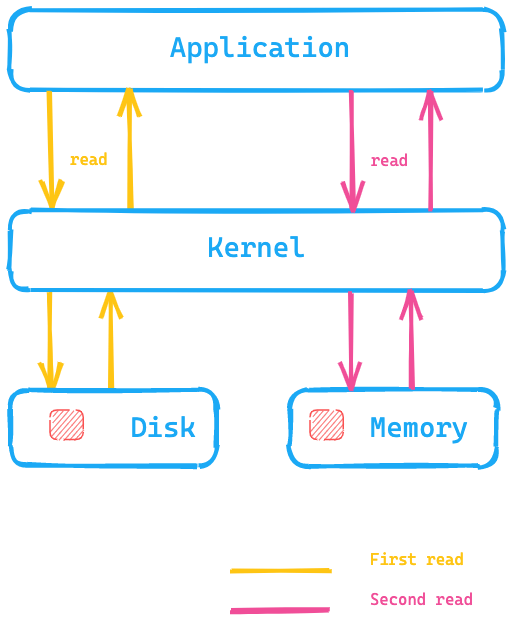
\includegraphics[width=0.5\textwidth]{chapter-2/cache-app.png}
    \caption{Prinsip Cache pada Aplikasi}
    \label{fig:cache-app}
\end{figure}

\begin{figure}[h]
    \centering
    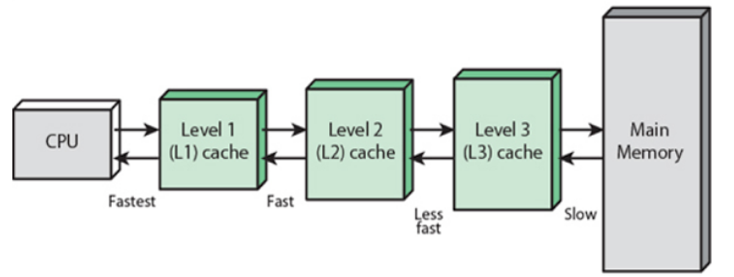
\includegraphics[width=0.5\textwidth]{chapter-2/cache-memory.jpeg}
    \caption{Level-level pada Cache}
    \label{fig:cache-level}
\end{figure}

\section{Kubernetes}

\subsection{Pod}
Pod adalah unit komputasi terkecil yang dapat dibuat dan dikelola dalam Kubernetes. Pod berisi lebih dari satu kontainer dan memiliki jaringan serta penyimpanan yang dipakai bersama serta spesifikasi untuk menjalankan kontainer didalamnya, \parencite{pod}.

\subsection{\textit{Autoscaler}}
\textit{Autoscaler} adalah komponen yang mengatur alokasi sumber daya komputasi secara dinamis yang disesuaikan dengan beban layanan pada saat tertentu. Saat ini di Kubernetes, terdapat dua pendekatan \textit{Autoscaling} 

\subsubsection{\textit{Horizontal Autoscaler}}
\textit{Horizontal Autoscaler} fokus untuk melakukan penskalaan dengan bantuan replikasi. \textit{Kubernetes Horizontal Pod Autoscaler} secara otomatis akan menlakukan penskalaan jumlah pod yang di-\textit{deploy} sehingga dapat menyesuaikan dengan kebutuhan dengan cara menambah atau mengurangi replikasi yang ada, \parencite{hpa}. 

\subsubsection{\textit{Vertical Autoscaler}}
Berbeda dengan cara horizontal, \textit{Vertical Autoscaler} lebih fokus untuk mengubah ukuran alokasi utilisasi pada pod yang ada. \textit{Kubernetes Vertical Pod Autoscaler} berguna untuk mengotomasi reservasi CPU dan memori yang sesuai. Penyesuaian ini dapat meningkatkan kluster kubernetes spesifiknya pada utilitasi sumber daya karena dapat mengurangi alokasi CPU dan memori pada sebuah \textit{node} agar bisa dipakai oleh pod lain, \parencite{vpa2}.

\subsection{\textit{Kubernetes Client Library}}
\textit{Kubernetes Client Library} adalah sebuah perpustakaan atau \textit{Library} yang dapat digunakan oleh \textit{developer} atau \textit{administrator} untuk berinteraksi dengan Kubernetes API \parencite{clientlibrary}. Saat ini, Kubernetes sudah memiliki \textit{library} resmi pada bahasa pemrograman, diantaranya.

\begin{enumerate}
    \item C (https://github.com/kubernetes-client/c),
    \item Dotnet (https://github.com/kubernetes-client/csharp),
    \item Golang (https://github.com/kubernetes/client-go/),
    \item Java (https://github.com/kubernetes-client/java),
    \item Python (https://github.com/kubernetes-client/python/),
    \item Haskell, Ruby, Perl, dan Javascript.
\end{enumerate}

Secara umum, beberapa fitur dari \textit{Kubernetes Client Library} antara lain sebagai berikut.
\begin{enumerate}
    \item Kemampuan untuk berinteraksi dengan berbagai jenis objek atau komponen pada \textit{cluster} Kubernetes, seperti pod, deployment, service, dan lain-lain.
    \item Fungsi untuk membuat, membaca, memperbarui, dan menghapus objek atau komponen pada \textit{cluster} Kubernetes.
    \item Melakukan autentikasi dan autorisasi pada API Kubernetes.
\end{enumerate}

\section{Prediksi Statistik}
Prediksi statistik adalah proses memprediksi nilai di masa depan dari suatu variabel berdasarkan data historis yang tersedia. Pendekatan statistik digunakan untuk memodelkan hubungan antara variabel-variabel yang berbeda dan untuk mengidentifikasi pola dan tren dalam data historis. Metode statistik yang umum digunakan untuk prediksi meliputi regresi dan analisis \textit{time series}.

Dalam prediksi statistik, model matematis dikembangkan untuk menggambarkan hubungan antara variabel input dan variabel output yang ingin diprediksi. Model ini akan digunakan untuk memperkirakan nilai variabel output berdasarkan nilai variabel input yang diberikan. Tujuannya adalah untuk menghasilkan prediksi yang akurat dengan menggunakan model yang dapat diuji dan diperbaiki berdasarkan data historis yang tersedia.

% Jelasin soal arima, sarima, etc
% Kasih referensi

% \section{Pembelajaran Mesin}
% Pembelajaran Mesin adalah sebuah bidang pembelajaran yang mempelajari pemahaman dan membangun metode untuk "belajar" dengan memanfaatkan data untuk meningkatkan banyak aspek terutama efisiensi dan kualitas terhadap suatu rangkaian tugas. Algoritma pembelajaran mesin membangun model berdasarkan data sampel yang biasa disebut \textit{training data} untuk menghasilkan model yang dapat memprediksi atau membuat keputusan tanpa diprogram secara eksplisit, \parencite{ml}.

% \subsection{\textit{Reinforcement Learning}}
% \textit{Reinforcement learning} atau RL adalah bidang pembelajaran mesin yang mengotomasi sebuah agen untuk mengambil tindakan dan memaksimalkan \textit{reward} dari aksi yang dilakukan, \parencite{reinforcementlearning}. RL adalah salah satu paradigma dari tiga pembelajaran mesin dasar seperti \textit{Supervised Learning} dan \textit{Unsupervised Learning}. Singkatnya, RL membuat agen dapat mengoreksi pengetahuannya secara terus menerus agar dapat memaksimalkan fungsinya. Berbeda dengan \textit{Supervised Learning}, RL tidak memerlukan label dan tidak memerlukan secara eksplisit dikoreksi. Fokus dalam membangun RL, adalah mencari keseimbangan eksplorasi terhadap lingkungan baru dan eksploitasi terhadap pengetahuan yang dimiliki.